\begin{pages}
    \begin{Rightside}
    \selectlanguage{greek}
        \beginnumbering
        \pstart[
        			\chapter{Ὁ ἐν τῇ ἡλίῳ ἑστηκὼς ἄγγελος}
        			\markboth{The Angel Standing in the Sun}
				]
		\renewcommand{\LettrineFontHook}{\PHtitl}
		\lettrine[lines=3]{Μ}{ετὰ} ταῦτα ἤκουσα ὡς φωνὴν μεγάλην ὄχλου πολλοῦ ἐν τῷ οὐρανῷ λεγόντων 	Ἁλληλουϊά· ἡ σωτηρία καὶ ἡ δόξα καὶ ἡ δύναμις τοῦ Θεοῦ ἡμῶν, ὅτι ἀληθιναὶ καὶ δίκαιαι αἱ κρίσεις αὐτοῦ· ὅτι ἔκρινεν τὴν πόρνην τὴν μεγάλην ἥτις ἔφθειρεν τὴν γῆν ἐν τῇ πορνείᾳ αὐτῆς, καὶ ἐξεδίκησεν τὸ αἷμα τῶν δούλων αὐτοῦ ἐκ χειρὸς αὐτῆς.
		\pend
		\pstart
		καὶ δεύτερον εἴρηκαν Ἁλληλουϊά· καὶ ὁ καπνὸς αὐτῆς ἀναβαίνει εἰς τοὺς αἰῶνας τῶν αἰώνων. καὶ ἔπεσαν οἱ πρεσβύτεροι οἱ εἴκοσι τέσσαρες καὶ τὰ τέσσερα ζῷα, καὶ προσεκύνησαν τῷ Θεῷ τῷ καθημένῳ ἐπὶ τῷ θρόνῳ λέγοντες Ἀμήν, Ἁλληλουϊά. καὶ φωνὴ ἀπὸ τοῦ θρόνου ἐξῆλθεν λέγουσα 	Αἰνεῖτε τῷ Θεῷ ἡμῶν, πάντες οἱ δοῦλοι αὐτοῦ, οἱ φοβούμενοι αὐτόν, οἱ μικροὶ καὶ οἱ μεγάλοι.
		\pend
		\pstart
		Καὶ ἤκουσα ὡς φωνὴν ὄχλου πολλοῦ καὶ ὡς φωνὴν ὑδάτων πολλῶν καὶ ὡς φωνὴν βροντῶν ἰσχυρῶν, λεγόντων Ἁλληλουϊά, ὅτι ἐβασίλευσεν Κύριος ὁ Θεός ἡμῶν ὁ Παντοκράτωρ. χαίρωμεν καὶ ἀγαλλιῶμεν, καὶ δώσομεν τὴν δόξαν αὐτῷ, ὅτι ἦλθεν ὁ γάμος τοῦ Ἀρνίου, καὶ ἡ γυνὴ 	αὐτοῦ ἡτοίμασεν ἑαυτήν, καὶ ἐδόθη αὐτῇ ἵνα περιβάληται βύσσινον λαμπρὸν καθαρόν· τὸ 	γὰρ βύσσινον τὰ δικαιώματα τῶν ἁγίων ἐστίν.
		\pend
		\pstart
		Καὶ λέγει μοι Γράψον Μακάριοι οἱ εἰς τὸ δεῖπνον τοῦ γάμου τοῦ Ἀρνίου κεκλημένοι. καὶ λέγει μοι Οὗτοι οἱ λόγοι ἀληθινοὶ τοῦ Θεοῦ εἰσιν. καὶ ἔπεσα ἔμπροσθεν τῶν ποδῶν αὐτοῦ προσκυνῆσαι αὐτῷ. καὶ λέγει μοι Ὅρα μή· σύνδουλός σού εἰμι καὶ τῶν ἀδελφῶν σου τῶν ἐχόντων τὴν μαρτυρίαν Ἰησοῦ· τῷ Θεῷ προσκύνησον· ἡ γὰρ μαρτυρία Ἰησοῦ ἐστιν τὸ πνεῦμα τῆς προφητείας. 
		\pend
		\pstart
		Καὶ εἶδον τὸν οὐρανὸν ἠνεῳγμένον, καὶ ἰδοὺ ἵππος λευκός, καὶ ὁ καθήμενος ἐπ’ αὐτὸν καλούμενος Πιστὸς καὶ Ἀληθινός, καὶ ἐν δικαιοσύνῃ κρίνει καὶ πολεμεῖ. οἱ δὲ ὀφθαλμοὶ αὐτοῦ φλὸξ πυρός, καὶ ἐπὶ τὴν κεφαλὴν αὐτοῦ διαδήματα πολλά, ἔχων ὄνομα γεγραμμένον ὃ οὐδεὶς οἶδεν εἰ μὴ αὐτός, καὶ περιβεβλημένος ἱμάτιον βεβαμμένον αἵματι, καὶ κέκληται τὸ ὄνομα αὐτοῦ Ὁ Λόγος τοῦ Θεοῦ. καὶ τὰ στρατεύματα τὰ ἐν τῷ οὐρανῷ ἠκολούθει αὐτῷ ἐφ’ ἵπποις λευκοῖς, ἐνδεδυμένοι βύσσινον λευκὸν καθαρόν. καὶ ἐκ τοῦ στόματος αὐτοῦ ἐκπορεύεται ῥομφαία ὀξεῖα, ἵνα ἐν αὐτῇ πατάξῃ τὰ ἔθνη· καὶ αὐτὸς ποιμανεῖ αὐτοὺς ἐν ῥάβδῳ σιδηρᾷ· καὶ αὐτὸς πατεῖ τὴν ληνὸν τοῦ οἴνου τοῦ θυμοῦ τῆς ὀργῆς τοῦ Θεοῦ τοῦ Παντοκράτορος. καὶ ἔχει ἐπὶ τὸ ἱμάτιον καὶ ἐπὶ τὸν μηρὸν αὐτοῦ ὄνομα γεγραμμένον ΒΑΣΙΛΕΥΣ ΒΑΣΙΛΕΩΝ ΚΑΙ ΚΥΡΙΟΣ ΚΥΡΙΩΝ. 
		\pend
		\pstart
		Καὶ εἶδον ἕνα ἄγγελον ἑστῶτα ἐν τῷ ἡλίῳ, καὶ ἔκραξεν ἐν φωνῇ μεγάλῃ λέγων πᾶσιν τοῖς ὀρνέοις τοῖς πετομένοις ἐν μεσουρανήματι Δεῦτε συνάχθητε εἰς τὸ δεῖπνον τὸ μέγα τοῦ Θεοῦ, ἵνα φάγητε σάρκας βασιλέων καὶ σάρκας χιλιάρχων καὶ σάρκας ἰσχυρῶν καὶ σάρκας ἵππων καὶ τῶν καθημένων ἐπ’ αὐτῶν, καὶ σάρκας πάντων ἐλευθέρων τε καὶ δούλων καὶ μικρῶν καὶ μεγάλων.
		\pend
		\pstart
		Καὶ εἶδον τὸ θηρίον καὶ τοὺς βασιλεῖς τῆς γῆς καὶ τὰ στρατεύματα αὐτῶν συνηγμένα ποιῆσαι τὸν πόλεμον μετὰ τοῦ καθημένου ἐπὶ τοῦ ἵππου καὶ μετὰ τοῦ στρατεύματος αὐτοῦ. καὶ ἐπιάσθη τὸ θηρίον καὶ μετ’ αὐτοῦ ὁ ψευδοπροφήτης ὁ ποιήσας τὰ σημεῖα ἐνώπιον αὐτοῦ, ἐν οἷς ἐπλάνησεν τοὺς λαβόντας τὸ χάραγμα τοῦ θηρίου καὶ τοὺς προσκυνοῦντας τῇ εἰκόνι αὐτοῦ· ζῶντες ἐβλήθησαν οἱ δύο εἰς τὴν λίμνην τοῦ πυρὸς τῆς καιομένης ἐν θείῳ. καὶ οἱ λοιποὶ ἀπεκτάνθησαν ἐν τῇ ῥομφαίᾳ τοῦ καθημένου ἐπὶ τοῦ ἵππου τῇ ἐξελθούσῃ ἐκ τοῦ στόματος αὐτοῦ, καὶ πάντα τὰ ὄρνεα ἐχορτάσθησαν ἐκ τῶν σαρκῶν αὐτῶν.	
		\pend
        \endnumbering
    \end{Rightside}
    \begin{Leftside}
        \beginnumbering
        \pstart[
        			\chapter{The Angel Standing in the Sun}
				]		
		\renewcommand{\LettrineFontHook}{\Zallmanfamily}
		\lettrine[lines=3]{H}{ereafter} I heard (something that was) like a great voice of a large crowd in Heaven saying, “Hallelujah. Salvation and glory and power of our God (be to God?), for his judgements are true and just; for he judged the great prostitute who corrupted the Earth in her sexual immorality and he has avenged the blood of his servants from (on?) her hand. 
		\pend
		\pstart
		And a second time they said “Hallelujah. And her smoke ascends into the eternity of eternities (forever).” And the twenty-four elders and the four creatures fell (to their knees?) and worshipped God — the One sitting upon the throne — saying, “Amen, Hallelujah”. And a voice came from the throne saying, “Praise our God — (you) all (who are) His servants and (who) fear Him; (both) the small and the great (shall praise Him).”
		\pend
		\pstart
		And I heard (something that was) as a voice of a great crowd and as a voice of many waters and as a voice of a vicious thunderstorm saying, “Hallelujah! For the Lord our God — the Almighty — has reigned. Let us rejoice and be glad and let us (also) give Him glory; for (there) has come the marriage of the Lamb and his wife has prepared herself and it was given to her (the honour?) to be clad in fine linen, bright and pure; for the fine linen are the righteous deeds of the holy men.” 
		\pend
		\pstart
		And he says to me, “Write (the following): ‘Blessed are those (who are) called to (attend) the feast of the Lamb’s marriage.’” And he tells me, “These true words are (those) of God.”. And I fell before his feet to worship him, but he says to me, “See not (i. e. do not do it); I am (one of) your fellow servant(s) and (I am one) of your brothers — (one) of those who have the witness of Jesus. Worship God, for the witness of Jesus is the spirit of (the) prophecy.”
		\pend
		\pstart
		And I saw Heaven open(ed), and look! A white horse and he who sits upon it is called Faithful and True; and in righteousness he judges and makes war. His eyes were (like?) a fiery flame and upon his head (there were) many crowns, having written (upon them) names which nobody — except him — knew. (And he was) clad in clothing dipped in blood, and he was called The Word of God by name. And his armies — those in Heaven — follow him on white horses (and they are all) clad in fine linen, pure and clean. And from his mouth there comes a sharp sword, so that he may strike the nations with it; and he shepherds them with a silver rod and tramples the winepress of the wrath of the anger (strong wrath?) of God the Almighty. And he has written upon his robe and his thigh the (following) name: “\textsc{The King of Kings and the Lord of Lords}”.
		\pend
		\pstart
		And I saw an angel standing in the Sun and he shouted in a great voice saying to all the birds (every bird) flying in mid-air, “Come (and) gather together (to go) to the great feast (supper, dinner) of God, so that you might eat the flesh of kings and the flesh of commanders and the flesh of strong (men) and the flesh of horses — and those who sit thereon — and the flesh of every free (man) and slave and (of everyone who is) small and great. 
		\pend
		\pstart
		And I saw the beast and the kings of the Earth and their armies gathering together (gathered together) to make war (fight) with the one sitting upon the horse and with his army. And the beast was seized (apprehended, caught) and with him the false prophets, the one who performed miracles before him, with which those who took the mark of the beast and those who worship its idol were deceived. (Whilst they were still) living, the two (of them) were thrown into the lake of fire burning with brimstone. And the remaining (ones) were killed by the sword, the one coming out of him who sits upon the horse; and all the birds were filled from their flesh. 
		\pend
        \endnumbering
    \end{Leftside}

\end{pages} 
\Pages

\clearpage
\thispagestyle{empty}
\null\vfill
\settowidth\longest{\huge\itshape […] and when I turned around I saw}
\begin{center}
\parbox{\longest}{%
  \raggedright{\huge\itshape%
    ``Quote here.'' \par\bigskip
  }
  \raggedleft\Large\MakeUppercase{``Scene from the Apocalypse'' — Francis Danby, 1829}\par%
}
\vfill\vfill
\clearpage\newpage
\end{center}
\newpage
\thispagestyle{empty}
\begin{center}
	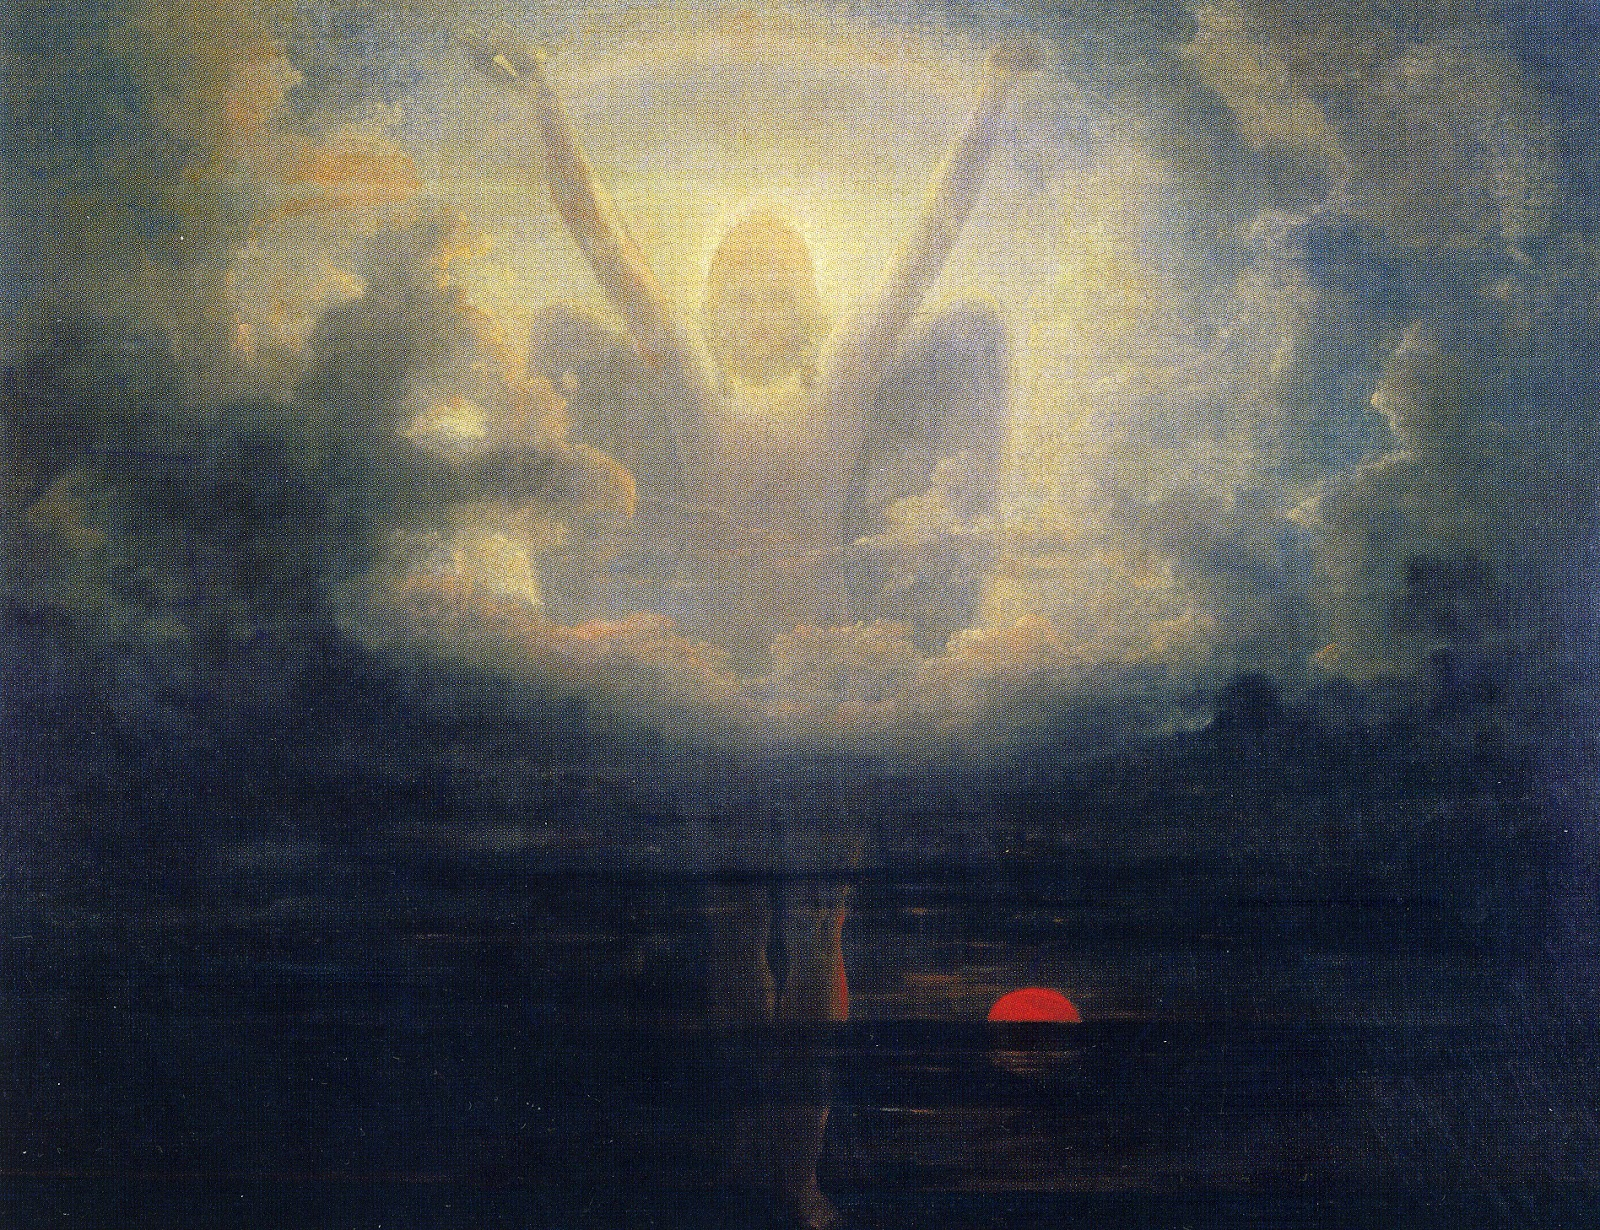
\includegraphics[angle=90, width=1\textwidth]{images/illustrations/danbyapocalypse}
\end{center}